\documentclass[]{ximera}
%handout:  for handout version with no solutions or instructor notes
%handout,instructornotes:  for instructor version with just problems and notes, no solutions
%noinstructornotes:  shows only problem and solutions

%% handout
%% space
%% newpage
%% numbers
%% nooutcomes

%I added the commands here so that I would't have to keep looking them up
%\newcommand{\RR}{\mathbb R}
%\renewcommand{\d}{\,d}
%\newcommand{\dd}[2][]{\frac{d #1}{d #2}}
%\renewcommand{\l}{\ell}
%\newcommand{\ddx}{\frac{d}{dx}}
%\everymath{\displaystyle}
%\newcommand{\dfn}{\textbf}
%\newcommand{\eval}[1]{\bigg[ #1 \bigg]}

%\begin{image}
%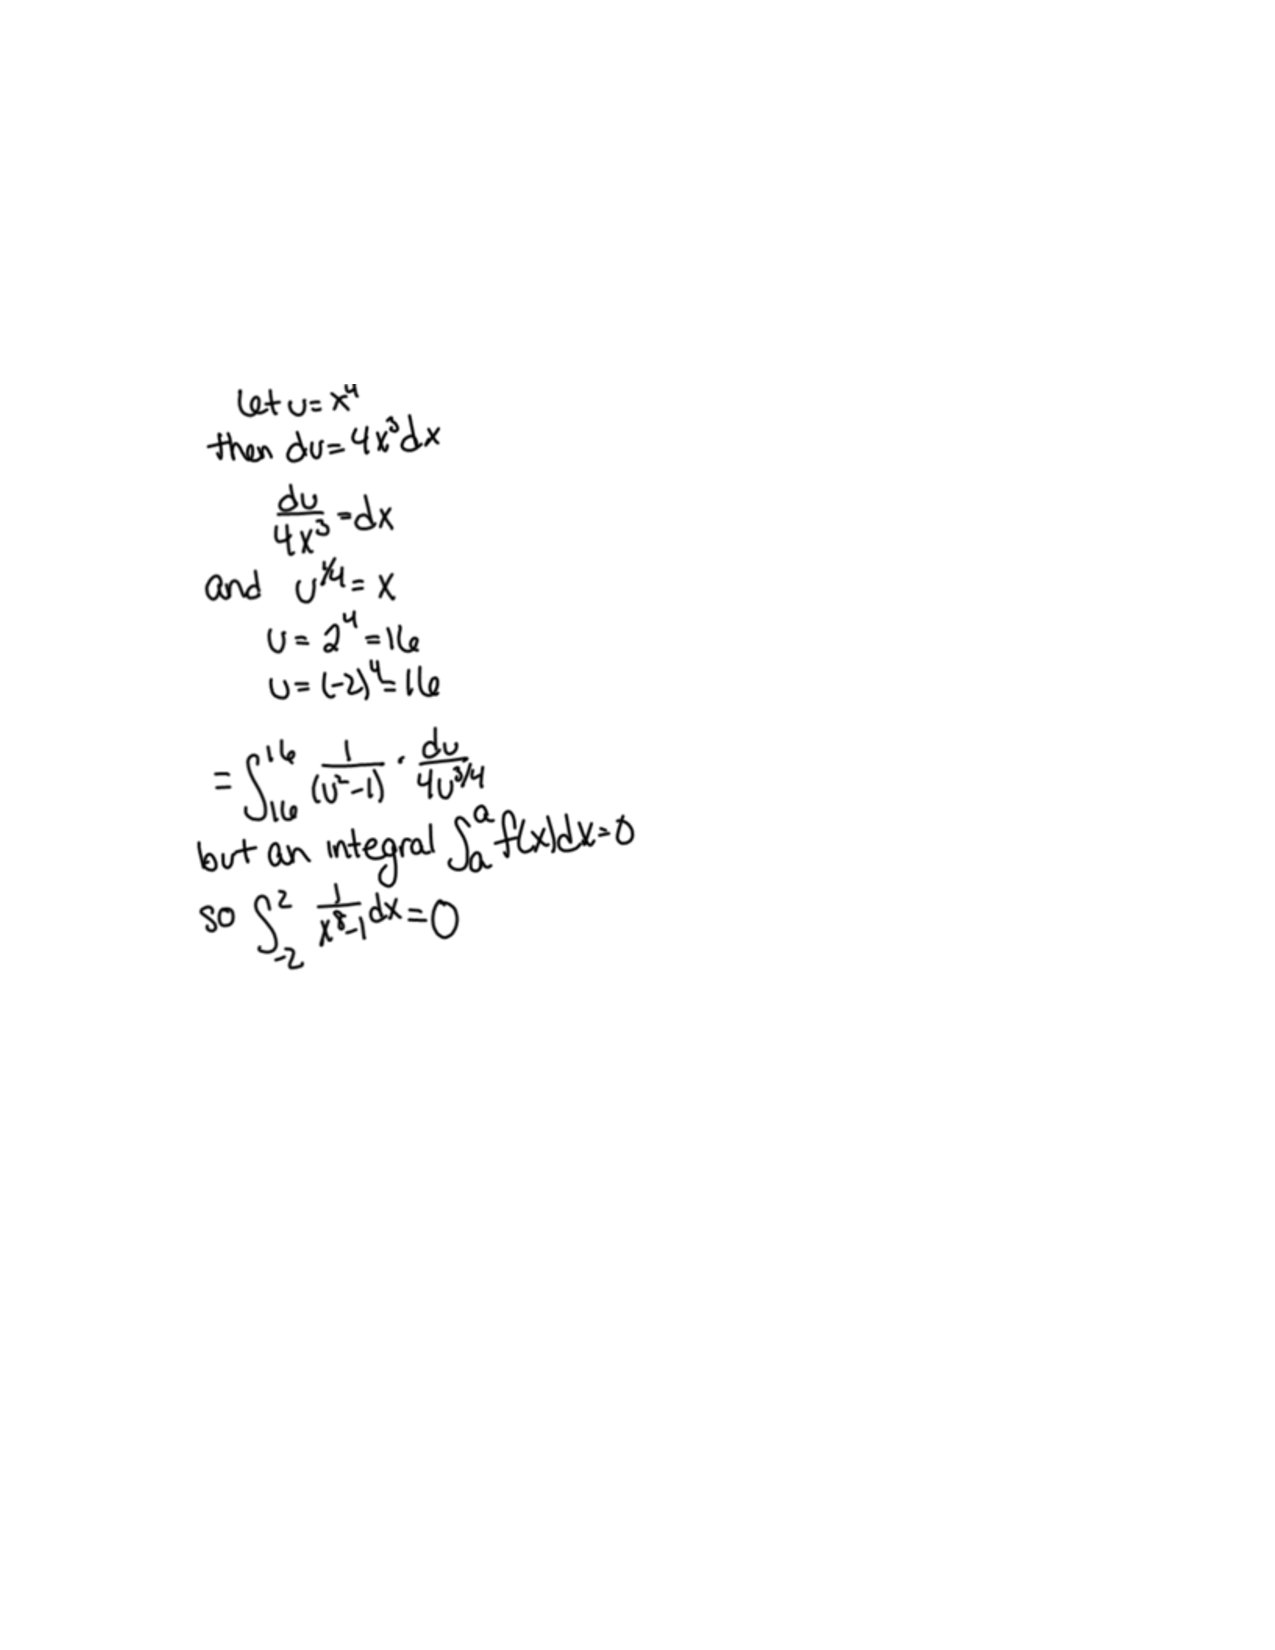
\includegraphics[trim= 170 420 250 180]{Figure1.pdf}
%\end{image}

%add a ``.'' below when used in a specific directory.
\newcommand{\RR}{\mathbb R}
\renewcommand{\d}{\,d}
\newcommand{\dd}[2][]{\frac{d #1}{d #2}}
\renewcommand{\l}{\ell}
\newcommand{\ddx}{\frac{d}{dx}}
\newcommand{\dfn}{\textbf}
\newcommand{\eval}[1]{\bigg[ #1 \bigg]}

\usepackage{multicol}

\renewenvironment{freeResponse}{
\ifhandout\setbox0\vbox\bgroup\else
\begin{trivlist}\item[\hskip \labelsep\bfseries Solution:\hspace{2ex}]
\fi}
{\ifhandout\egroup\else
\end{trivlist}
\fi} %% we can turn off input when making a master document

\title{Parametric equations}  

\begin{document}
\begin{abstract}		\end{abstract}
\maketitle



\section{Warm up:}
Describe the motion given by $x=8$, $y=7 \sin (t)$ for all $t$.
	\begin{freeResponse}
	The parametric curve keeps oscillating up and down the vertical line segment between the points $(8,-7)$ and $(8,7)$.
	This is because $x=8$ is fixed, and $y = 7 \sin(t)$ oscillates between $-7$ and $7$ as $t$ varies.
	\end{freeResponse}
	
\begin{instructorNotes}
One variable is held constant while the other oscillates up and down.
\end{instructorNotes}







\section{Group work:}



%problem 1
\begin{problem}
Try to figure out the shape of the following curve and then eliminate the parameter and check your intuition.
	\[
	x = \ln t - 1 \qquad y = \ln^2 t
	\]
	\begin{freeResponse}
	First, note that these two functions are both only defined when $0 < t < \infty$.  
	Also, we see that $\ln t = x + 1$, and so 
		\[
		y = \ln^2 t = (x+1)^2.
		\]
	So this graph is a parabola that opens up and has vertex $(-1,0)$.  
	
	\begin{image}
	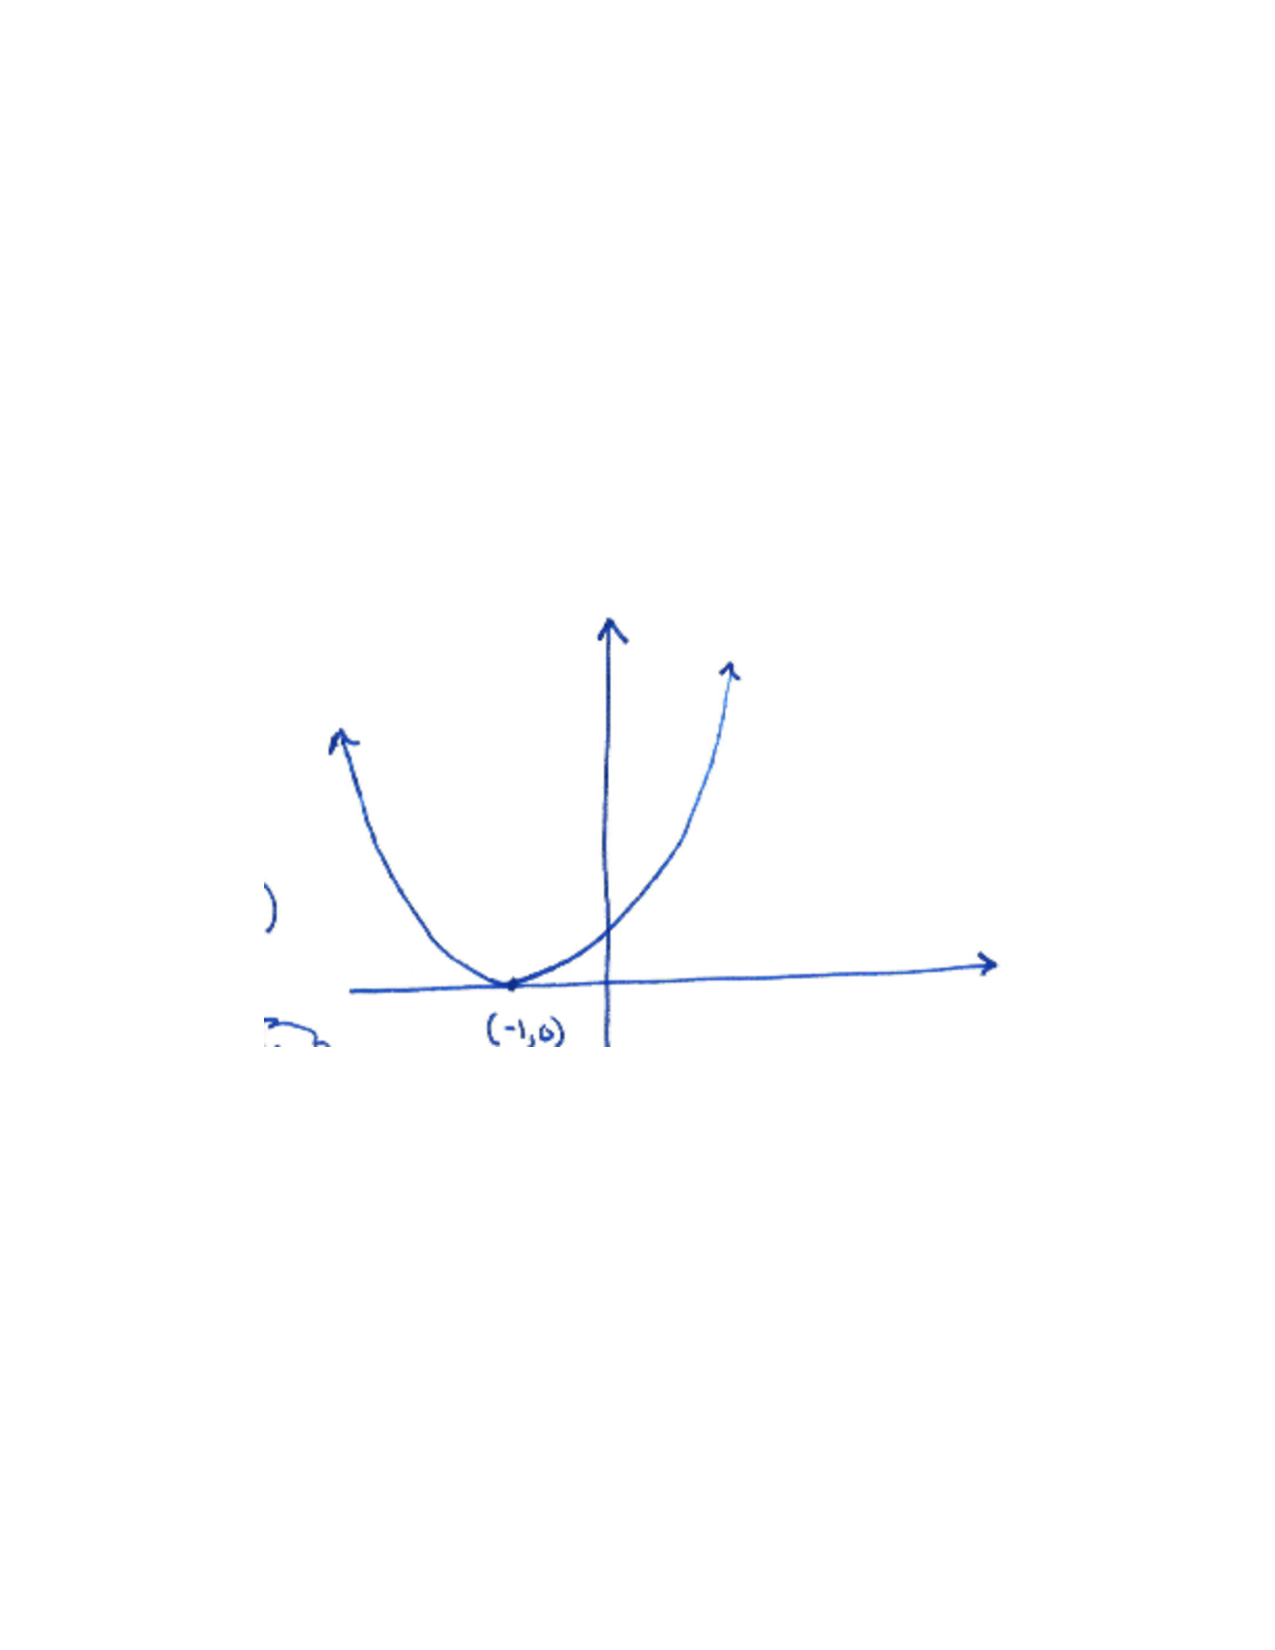
\includegraphics[trim= 170 270 170 310]{Figure11-1-1.pdf}
	\end{image}
	\end{freeResponse}
	
\end{problem}

\begin{instructorNotes}
It is not hard to see that $y = (x+1)^2$.  
So this is a parabola.  
\end{instructorNotes}







%problem 2
\begin{problem}
Find parametric equations for the path of a particle moving around the circle
	\[
	(x-3)^2 + (y+7)^2 = 4
	\]
	
	\begin{enumerate}
	\item  one time around clockwise starting at $(5,-7)$.  
	\item  three times around counterclockwise starting at $(5,-7)$.  
	\item  halfway around clockwise starting at $(-1,-7)$.  
	\end{enumerate}
	
	\begin{freeResponse}
	First, notice that this is the equation of the circle with radius $2$ centered at $(3,-7)$.  
	\begin{enumerate}
	\item  The point $(5,-7)$ is the ``right-most'' point on the circle.  
	In order to parameterize the circle one time around going {\it counter-clockwise} we use the parameterization
		\[
		x = 3 + 2 \cos t 	\qquad 	y = -7 + 2 \sin t 	\qquad	0 \leq t < 2 \pi.
		\]
	In order to traverse the circle one time {\it clockwise}, we just negate the $t$ in the above parameterization.  
	So we get
		\[
		\boxed{x = 3 + 2 \cos(-t) 	\qquad	y = -7 + 2 \sin(-t) 	\qquad	0 \leq t < 2 \pi}.
		\]
	{\it Remark:  Since $\cos$ is an even function and $\sin$ is an odd function, this solution is equivalent to
		\[
		x = 3 + 2 \cos t 	\qquad	y = -7 - 2 \sin t 	\qquad	0 \leq t < 2 \pi
		\]
	}
	
	
	
	\item  To traverse the circle three times counter-clockwise, we just triple the domain of $t$ from the parameterization above.  
	So we have that
		\[
		\boxed{x = 3 + 2 \cos t 	\qquad 	y = -7 + 2 \sin t 	\qquad	0 \leq t < 6 \pi}.
		\]
	
	
	
	\item  Note that this problem starts at $(-1,-7)$, not $(5,-7)$.  
	So this parameterization begins at the ``left-most'' point of the circle.  
	Therefore, this is just the ``second half'' of the answer to part (a).  
	So a parameterization for this problem is
		\[
		\boxed{x = 3 + 2 \cos(-t) 	\qquad	y = -7 + 2 \sin(-t) 	\qquad	\pi \leq t < 2 \pi}.
		\]
	
	\end{enumerate}
	\end{freeResponse}
		
\end{problem}

\begin{instructorNotes}
Practice with the formula for parameterizing a circle.  
It is useful to point out that the same curve can have many different parameterizations.
\end{instructorNotes}







%problem 3
\begin{problem}
Find the intersection point(s) of the lines
	\begin{equation}\label{line 1}
	x=-6 + 9t, 	\qquad 	y = 3-2t
	\end{equation}
and
	\begin{equation}\label{line 2}
	x=3+t, 	\qquad	y=-4-2t.
	\end{equation}
Do they intersect at the same time?
	\begin{freeResponse}
	Line \ref{line 1} is the line with slope $- \frac{2}{9}$ passing through $(-6,3)$.  
	So it has equation
		\begin{align*}
		&y - 3 = - \frac{2}{9} (x-(-6))  \\
		\Longrightarrow 	\qquad 	&y = - \frac{2}{9} x - \frac{4}{3} + 3 = - \frac{2}{9} x + \frac{5}{3}.
		\end{align*}
		
	Line \ref{line 2} is the line with slope $- 2$ passing through $(3,-4)$.  
	So it has equation
		\begin{align*}
		&y + 4 = -2 (x- 3)  \\
		\Longrightarrow 	\qquad 	&y = - 2x + 2.
		\end{align*}
		
	Since these lines have different slopes, they intersect in a single point.  
	To find this point, we set the equations equal to each other:
		\begin{align*}
		&- \frac{2}{9} x + \frac{5}{3} = -2x+2  \\
		\Longrightarrow 	\qquad 	&\frac{16}{9} x = \frac{1}{3}  \\
		\Longrightarrow 	\qquad 	&x = \frac{3}{16}  \\
		\Longrightarrow 	\qquad 	&y = -2 \left( \frac{3}{16} \right) + 2 = \frac{13}{8}.
		\end{align*}
	Therefore, the intersection point is
		\[
		\boxed{ \left( \frac{3}{16}, \frac{13}{8} \right)}.
		\]
		
	To see if they intersect in the same point, let us first find the $t$ value which makes the $x$-coordinate of line \ref{line 1} equal to $\frac{3}{16}$.  
		\begin{align*}
		&\frac{3}{16} = -6 + 9t  \\
		\Longrightarrow 	\qquad 	&t = \frac{1}{9} \left( \frac{3}{16} + 6 \right) = \frac{11}{16}.
		\end{align*}
	So now, we plug this into the equation for $x(t)$ for line \ref{line 2} and see if we get $\frac{3}{16}$.
		\begin{align*}
		x \left( \frac{11}{16} \right) &= 3 + \frac{11}{16}  \\
		&= \frac{59}{16} \neq \frac{3}{16}.
		\end{align*}
	Therefore, these lines do {\bf not} intersect at the same time.
	\end{freeResponse}

\end{problem}

\begin{instructorNotes}
The key point here is that intersections can occur at different ``times''.
\end{instructorNotes}







%problem 4
\begin{problem}
Consider the curve defined by the parameterization $x=t^2$, $y= t^3 - 3t$.  
Show that this curve has two tangent lines at $(3,0)$, and find the equations of the tangent lines there.
	\begin{freeResponse}
	First, recall that
		\[
		\frac{\d y}{\d x} = \frac{\frac{\d y}{\d t}}{\frac{\d x}{\d t}}.
		\]
	Then, since $\frac{\d x}{\d t} = 2t$ and $\frac{\d y}{\d t} = 3t^2 - 3$, we have that
		\[
		\frac{\d y}{\d x} = \frac{3t^2 - 3}{2t}.
		\]
	Now,
		\begin{align*}
		&x(t) = 3  \\
		\Longleftrightarrow 	\qquad	&t^2 = 3  \\
		\Longleftrightarrow 	\qquad	&t = \pm \sqrt{3}.
		\end{align*}
	Also, notice that both $y(\sqrt{3}) = 0 = y(- \sqrt{3})$.  
	So the given parametric curve intersects the point $(3,0)$ at two times, when $t = \pm \sqrt{3}$.  
	At these two times, the tangent lines have slopes
		\[
		\frac{\d y}{\d x} \biggr|_{t = \sqrt{3}} = \frac{(3)(3) - 3}{2 \sqrt{3}} = \sqrt{3}	\qquad	\text{and}	\qquad	\frac{\d y}{\d x} \biggr|_{t = - \sqrt{3}} = \frac{(3)(3) - 3}{-2 \sqrt{3}} = -\sqrt{3}.
		\]
	So the equations of the tangent lines are
		\begin{align*}
		&\boxed{y = \sqrt{3} (x-3)}  \\
		&\boxed{y = -\sqrt{3}(x-3)}.
		\end{align*}
	\end{freeResponse}

\end{problem}

\begin{instructorNotes}
The main idea here is that a parametric curve can have several tangent lines at the same point (in $(x,y)$ coordinates).
\end{instructorNotes}
















	
	
	
	
	
	
	
	
	

	










								
				
				
	














\end{document} 


















